\documentclass[journal]{IEEEtran}

% ===== XeLaTeX / Unicode 字体路线 =====
\usepackage{iftex}
\ifXeTeX
  \usepackage{fontspec}
  \usepackage{xeCJK}
  \usepackage{amsmath}
  \usepackage{unicode-math}
  \usepackage{algorithm}
  \usepackage{algorithmic}

  % 关键：延后覆盖 IEEEtran 的 ptm 设置，避免 TU/ptm 报错
  \AtBeginDocument{%
    % 正文字体
    \setmainfont{TeX Gyre Termes}
    \setsansfont{TeX Gyre Heros}
    \setmonofont{JetBrains Mono}
    \setCJKmainfont{Noto Serif CJK SC}[BoldFont=Noto Serif CJK SC]

    % 数学字体
    \setmathfont{TeX Gyre Termes Math}
  }
\else
  % 如果不是 XeLaTeX（比如 pdfLaTeX），这里可以放兼容方案或直接报错
\fi

% ===== 常用宏包 =====
\usepackage{graphicx}
\usepackage{booktabs}
\usepackage{cite}

\begin{document}
\title{Weakly Supervised Early Warning of Conflict Escalation in Social Media Comment Streams}

\author{Linli~Zhu\ (朱林立)\IEEEauthorrefmark{1}, Ziqiang~Ma\ (马自强)\IEEEauthorrefmark{2}%
\thanks{Manuscript received Month DD, YYYY; revised Month DD, YYYY.}%
\thanks{\IEEEauthorrefmark{1}L. Zhu is with the School of Computer Science, Ningxia University, Yinchuan, China (e-mail: violina2333@gmail.com).}%
\thanks{\IEEEauthorrefmark{2}Z. Ma is with the School of Information Engineering, Ningxia University, Yinchuan, China (e-mail: maziqiang@nxu.edu.cn). Corresponding author: L. Zhu.}}

\maketitle

\begin{abstract}
Social media discussions can escalate rapidly, making early identification of risky public-opinion dynamics important for timely intervention. Existing studies often focus on classifying sentiment or harmfulness at the level of individual posts, but they provide limited support for forecasting how topic-level conflict evolves over time. In this paper, we propose a weakly supervised framework for early warning of conflict escalation in social-media comment streams. The framework first computes a comment-level conflict index by combining interpretable signals of antagonistic intensity, negative high-arousal emotion, and stance polarization, without requiring manual annotation. These post-level scores are then aggregated into bin-level topic risk trajectories, which are modeled by a CNN-BiLSTM forecaster to predict short-horizon future risk under streaming conditions. Based on the predicted trajectory, a set of practical trigger rules is further introduced to issue early warnings according to threshold exceedance, rapid growth, persistence, and tail-risk amplification. The proposed framework aims to bridge fine-grained text signals and temporal public-opinion monitoring in an interpretable manner. Experimental evaluation demonstrates its potential for identifying emerging escalation trends and supporting proactive intervention in online public-opinion governance.
\end{abstract}

\begin{IEEEkeywords}
conflict index, early warning, social media comments, public opinion surveillance, temporal forecasting, LSTM, weakly supervised learning, stance polarization
\end{IEEEkeywords}

\section{Introduction}

\subsection{Challenges in Governing Social Media Public Opinion}
The ubiquity of social media has transformed how information is produced, circulated, and contested. Public debates that once unfolded over days now escalate within hours as platforms enable rapid information cascades and viral diffusion~\cite{Vosoughi2018}. Seemingly marginal topics can ignite large-scale opinion swings with tangible offline consequences. For example, coordinated online discourse has been shown to correlate with mass protests and even violent incidents in subsequent days~\cite{Steinert2015,Arcila2024}. 

\subsubsection{Information Cascades and Offline Spillovers}
Information spreads faster than it can be verified. Emotional contagion and algorithmic amplification jointly fuel cascades that can spill over into offline actions. Once critical mass is reached, moderation or fact-checking becomes less effective, as narratives solidify through repeated exposure~\cite{Vosoughi2018}. These cascades thus demand proactive, not reactive, management.

\subsubsection{Delays in Post-hoc Sentiment Analysis}
Conventional sentiment analysis frameworks primarily offer retrospective insight: they describe how people felt after events unfolded. However, by the time significant polarity shifts are detected, the discussion may already have escalated beyond control. This latency between event occurrence and analytical response undermines the capacity for early intervention~\cite{Wang2020}.

\subsubsection{Research Gaps in Early Warning}
Despite advances in opinion mining and social listening, few studies explicitly target early warning. Existing tools classify emotions or toxicity per message, but rarely attempt to forecast when online discontent is likely to escalate~\cite{Wang2020}. This absence of anticipatory modeling creates a crucial gap between detection and prevention.

\subsection{Limitations of Existing Technical Paradigms}

\subsubsection{Lexicon/Rule-Based Systems: Cross-Language and Sarcasm Fragility}
Lexicon-based or rule-driven systems offer interpretability but struggle with context-dependent semantics, sarcasm, and multilingual variation. Irony (“Great, another perfect policy!”) or cultural idioms can easily invert meaning~\cite{Dhumpati2025}. Moreover, such systems require language-specific dictionaries that fail in cross-lingual or code-mixed environments~\cite{Kaity2020}.

\subsubsection{Static Classifiers: Concept Drift and Out-of-Distribution Failure}
Traditional supervised classifiers, like \emph{SVM} or \emph{CNN}, are trained on fixed datasets and assume distributional stability. In dynamic online environments, vocabulary, sentiment norms, and social topics evolve rapidly—an issue known as concept drift~\cite{Gama2014}. Without continuous adaptation, static models degrade, misclassify emergent patterns, or fail to generalize to unseen contexts.

\subsubsection{Post-Level Semantic Analysis without Temporal Escalation Modeling}
Recent pretrained language models and text analysis systems substantially improve post-level semantic understanding, sentiment recognition, and harmful-content detection. However, these methods are often used to score or classify comments independently, without explicitly modeling how conflict accumulates and evolves across time. Consequently, they provide informative local signals but limited support for topic-level escalation forecasting and early warning. This motivates the introduction of a temporal forecasting layer on top of interpretable post-level risk signals~\cite{Abdalgader2025}.

\subsection{Contributions of This Work}

To address the above limitations, we propose a weakly supervised framework for topic-level conflict escalation monitoring and early warning in social-media comment streams. Rather than relying on manually annotated escalation labels, the framework first constructs an interpretable conflict signal at the comment level and then models its temporal evolution for short-horizon forecasting. The main contributions of this paper are as follows:

\noindent\textbf{(I-C1) Conflict-index quantification framework (Sec.~III-B):}
We introduce a weakly supervised \emph{conflict index} that quantifies antagonistic cues in social-media comments by combining attack-related intensity, negative high-arousal emotion, and stance polarization into a unified post-level score. This design provides an interpretable bridge between raw text and temporal risk modeling without requiring manual labels.

\noindent\textbf{(I-C2) Topic-level temporal forecasting via bin-level risk trajectories (Sec.~\ref{sec:lstm_forecast}):}
We aggregate comment-level conflict scores into bin-level topic risk trajectories and use a CNN-BiLSTM hybrid forecaster to model persistence, volatility, and rising trends. This enables short-horizon prediction of future topic risk under streaming conditions.

\noindent\textbf{(I-C3) Practical early-warning trigger rules (Sec.~III-D):}
We further design a set of trigger rules based on threshold exceedance, rapid growth, persistence, and tail-risk amplification, translating predicted trajectories into actionable early-warning decisions for public-opinion surveillance and intervention.

\subsection{Paper Structure Overview}
The remainder of this paper is organized as follows. Section~II reviews related studies in sentiment analysis, harmful content detection, and temporal modeling. Section~III presents the proposed framework, including the conflict-index formulation, CNN-BiLSTM temporal forecasting, and early-warning trigger rules. Section~IV outlines the experimental design and research questions, followed by concluding remarks and future directions.

\section{Related Work}

\subsection{Deep Learning for Sentiment and Emotion Understanding}
Deep learning has significantly advanced sentiment analysis by learning contextual and compositional linguistic patterns that are difficult to encode with lexicon-based rules or handcrafted features. A recent survey in~\cite{pimpalkar2025sentiment} traces this evolution from classical approaches to neural architectures, highlighting how LSTMs, CNNs, and Transformer encoders (e.g., BERT and GPT-style models) improve classification accuracy through representation learning. Despite these gains, key challenges remain, including robustness to sarcasm and irony, domain shift across platforms and topics, multilingual and code-mixed text processing, and the need for explainable sentiment reasoning for high-stakes governance applications~\cite{pimpalkar2025sentiment}. These limitations motivate models that (i) provide interpretable intermediate signals and (ii) remain effective under rapidly changing discourse.

\subsection{Risk Scoring for Harmful Content and Hazardous Conversations}
Beyond categorical sentiment labels, risk scoring aims to assign continuous severity estimates to online comments to support scalable moderation and hazard monitoring. Wulczyn \emph{et al.}~\cite{Wulczyn2017} construct a large corpus of Wikipedia discussion comments annotated for personal attacks and train predictive models that output, for each comment, the probability of being an attack. Such probabilistic outputs serve as practical risk scores for triage and prioritization, enabling moderators to focus on high-risk items and to identify discussion spaces with elevated aggression. However, most risk-scoring systems remain \emph{instance-centric}: they optimize snapshot detection at the comment level and treat posts as independent samples. As a result, they do not explicitly characterize how risk accumulates and propagates within a topic over time, nor do they naturally support trajectory-level forecasting and early warning. The conflict-index formulation in this paper builds on the idea of continuous risk scoring while explicitly designing the score to be both post-level interpretable and suitable as a temporal signal for escalation modeling.

\subsection{Temporal Forecasting of Public Opinion Trends with LSTM Variants}
Forecasting public opinion dynamics during emergencies requires temporal models that can capture persistence, volatility, and bursty surges in online activity. LSTM-based predictors are widely adopted for such sequence modeling, but their performance can be sensitive to hyperparameter choices under highly nonlinear and nonstationary trends. To improve forecasting stability, Mu \emph{et al.}~\cite{Mu2023IPSO} propose an Improved Particle Swarm Optimization LSTM (IPSO--LSTM) framework that uses adaptive search strategies (e.g., nonlinearly decreasing inertia weights and mutation mechanisms) to tune LSTM hyperparameters and avoid poor local optima. Their results show improved error metrics (e.g., MAPE and RMSE) relative to standard LSTM variants on multiple emergency-event datasets~\cite{Mu2023IPSO}. While these studies demonstrate the value of enhanced temporal predictors, they typically operate on aggregate time series and do not incorporate fine-grained, post-level semantic evidence. Our work complements this line of research by coupling contextual language understanding (via sentence-embedding-derived conflict signals) with temporal sequence modeling (via LSTM) to produce interpretable, topic-level escalation trajectories and short-horizon early warnings.

\section{Conflict-Index Formulation and CNN-BiLSTM Forecasting Framework}

\subsection{Problem Definition}

We study social-media comment streams organized by topic and discretized into fixed-length time bins. For a given topic, let the observation period be partitioned into $T$ consecutive bins of equal duration. For notation simplicity, we omit the topic index in the following definitions. Denote by $\mathcal{B}_t = \{x_{t,i}\}_{i=1}^{n_t}$ the multiset of $n_t$ comments posted in bin $t \in \{1, \dots, T\}$, where each $x_{t,i}$ represents a text message.

Our first objective is to assign an interpretable \emph{conflict index} to each comment via a text encoder $f_\theta$:
\begin{equation}
c_{t,i} = f_\theta(x_{t,i}) \in [0, 1],
\end{equation}
where higher values indicate stronger antagonistic cues (e.g., high-arousal negative emotion and confrontation markers). To obtain a topic-level risk signal per bin, we aggregate comment-level indices using a fixed aggregation operator $\mathrm{Agg}(\cdot)$:
\begin{equation}
\bar{c}_t = \mathrm{Agg}\left(\{c_{t,i}\}_{i=1}^{n_t}\right) \in [0, 1].
\end{equation}

Our second objective is early warning through short-horizon forecasting. Given the historical binned sequence $\bar{c}_{1:t}$, we learn a temporal predictor $g_\phi$ to estimate the future risk trajectory $\mathbf{\hat{c}}$ over a horizon $H$:
\begin{equation}
\mathbf{\hat{c}}_{t+1:t+H} = g_\phi(\bar{c}_{1:t}).
\end{equation}
An escalation warning is triggered at time bin $t$ if the predicted risk is expected to exceed a predefined threshold $\eta$ within the horizon, i.e.,
\begin{equation}
\max_{1 \le h \le H} \hat{c}_{t+h} \ge \eta,
\end{equation}
optionally combined with a rapid-growth criterion to capture fast-rising trends.

\subsection{Conflict-Index Quantification without Manual Labels}\label{sec:conflict_index}

Our dataset contains only time-stamped comment text streams and provides no human-annotated labels. We therefore construct an unsupervised (weakly supervised) \emph{conflict index} by combining three interpretable components: (i) antagonistic/attack intensity, (ii) negative high-arousal emotion intensity, and (iii) stance polarization derived from within-bin semantic bimodality. For each comment $x_{t,i}$ posted in time bin $t$, we compute
\begin{equation}
c_{t,i} = \sigma\!\left(w_a \tilde{a}_{t,i} + w_e \tilde{e}_{t,i} + w_s \tilde{s}_{t,i} + b\right)\in[0,1],
\label{eq:conflict_index_fusion}
\end{equation}
where $\sigma(\cdot)$ is the sigmoid function, $w_a,w_e,w_s \ge 0$ control the relative contributions (e.g., $w_a:w_e:w_s = 0.5:0.3:0.2$), and $b$ is a bias term. The tildes denote \emph{distribution-calibrated} scores (Sec.~\ref{sec:calibration}) so that components from different sources become comparable.

\subsubsection{Attack/Antagonism Intensity from a Pretrained Harm Model}
We obtain an antagonism score from a pretrained harmful/attack detector (e.g., toxicity/insult/hate model) that outputs a probability of attack-like content for a given text:
\begin{equation}
a_{t,i} = h_{\psi}(x_{t,i}) \in [0,1],
\label{eq:attack_score}
\end{equation}
where $h_{\psi}$ is a frozen pretrained model. This score serves as a \emph{pseudo-label prior} capturing confrontation markers, threats, harassment, and abusive language without requiring any task-specific annotation.

\subsubsection{Emotion Intensity from a Zero-Shot Emotion Model}
We characterize emotionally charged negativity using a zero-shot (or pretrained) emotion model that produces probabilities for emotion categories. Let $p_{\text{neg}}(x_{t,i})$ denote the probability of negative sentiment and $p_{\text{anger}}(x_{t,i})$ denote the probability of anger (a high-arousal negative emotion). We define
\begin{equation}
e_{t,i} = \alpha\, p_{\text{neg}}(x_{t,i}) + (1-\alpha)\, p_{\text{anger}}(x_{t,i}), \quad \alpha \in [0,1],
\label{eq:emotion_score}
\end{equation}
where $\alpha$ balances general negativity and arousal-related anger (we use $\alpha\in[0.6,0.8]$ in practice). This construction rewards comments that are both negative and emotionally intense, which are common precursors to conflict escalation.

\subsubsection{Stance Polarization via Within-Bin Semantic Bimodality}
In the absence of stance labels (pro/con/neutral), we estimate polarization by measuring whether comments within the same time bin form two semantically separated camps. We first compute sentence embeddings using a frozen encoder $\mathrm{Enc}(\cdot)$ (e.g., multilingual BERT pooling or sentence-transformer):
\begin{equation}
\mathbf{v}_{t,i} = \mathrm{Enc}(x_{t,i}) \in \mathbb{R}^d.
\label{eq:embedding}
\end{equation}
Within bin $t$, we apply $k{=}2$ clustering (e.g., k-means) on $\{\mathbf{v}_{t,i}\}_{i=1}^{n_t}$ to obtain two cluster centroids $\mathbf{u}_{t,1}$ and $\mathbf{u}_{t,2}$. The inter-camp separation is measured by
\begin{equation}
\Delta_t = 1 - \cos(\mathbf{u}_{t,1}, \mathbf{u}_{t,2}) \in [0,2],
\label{eq:camp_separation}
\end{equation}
where $\cos(\cdot,\cdot)$ is cosine similarity. Next, we quantify how strongly each comment aligns with one camp over the other. Let $d(\cdot,\cdot)$ be a distance function (we use cosine distance). Define the camp-alignment confidence
\begin{equation}
q_{t,i} = \frac{\left|d(\mathbf{v}_{t,i},\mathbf{u}_{t,1}) - d(\mathbf{v}_{t,i},\mathbf{u}_{t,2})\right|}
{d(\mathbf{v}_{t,i},\mathbf{u}_{t,1}) + d(\mathbf{v}_{t,i},\mathbf{u}_{t,2}) + \epsilon} \in [0,1],
\label{eq:alignment_confidence}
\end{equation}
with a small $\epsilon>0$ to avoid division by zero. Finally, the stance polarization score for a comment is
\begin{equation}
s_{t,i} = \mathrm{norm}(\Delta_t)\cdot q_{t,i} \in [0,1],
\label{eq:stance_score}
\end{equation}
where $\mathrm{norm}(\Delta_t)$ maps the separation magnitude to $[0,1]$ (e.g., $\mathrm{norm}(\Delta_t)=\min(1,\Delta_t)$). This assigns higher polarization to bins that exhibit two distinct camps and to comments that are clearly affiliated with one camp.

\subsubsection{Distribution Calibration by Percentile Mapping}\label{sec:calibration}
Scores produced by different pretrained models and heuristics can have inconsistent scales and distributions. We therefore calibrate each raw component score using an empirical cumulative distribution function (ECDF) computed over the entire corpus (or a large subset). For a raw score $r_{t,i}\in[0,1]$ (standing for $a_{t,i}$, $e_{t,i}$, or $s_{t,i}$), we define
\begin{equation}
\tilde{r}_{t,i} = \mathrm{ECDF}_r(r_{t,i}) \in [0,1],
\label{eq:ecdf}
\end{equation}
which maps $r_{t,i}$ to its percentile rank. This calibration yields comparable $\tilde{a}_{t,i},\tilde{e}_{t,i},\tilde{s}_{t,i}$ for fusion in (\ref{eq:conflict_index_fusion}).

\subsubsection{Bin-Level Aggregation for Topic Risk Trajectories}
To obtain a topic-level risk signal per time bin, we aggregate comment-level indices $\{c_{t,i}\}_{i=1}^{n_t}$ in a way that emphasizes the high-risk tail (since a small fraction of highly antagonistic comments may drive escalation). Let $c^{(1)}_t \ge \cdots \ge c^{(n_t)}_t$ be the sorted indices in bin $t$. We use a top-$k$ mean:
\begin{equation}
\bar{c}_t = \frac{1}{k}\sum_{j=1}^{k} c^{(j)}_t,\qquad k=\left\lceil \rho n_t \right\rceil,
\label{eq:topk_agg}
\end{equation}
where $\rho\in[0.05,0.2]$ controls the fraction of highest-risk comments included. The resulting $\{\bar{c}_t\}_{t=1}^T$ forms a smooth, interpretable risk trajectory that serves as input to the temporal predictor in Sec.~\ref{sec:lstm_forecast}.

\begin{algorithm}[t]
\caption{Unsupervised Conflict Index Computation}\label{alg:conflict_index}
\begin{algorithmic}[1]
\REQUIRE Comments $\{x_{t,i}\}$ grouped into bins $\mathcal{B}_t$; pretrained harm model $h_\psi$; zero-shot emotion model $g_\omega$; embedding encoder $\mathrm{Enc}$; top fraction $\rho$
\ENSURE Comment-level indices $\{c_{t,i}\}$ and bin-level trajectory $\{\bar c_t\}$
\FOR{$t=1$ to $T$}
  \FOR{each comment $x_{t,i}\in\mathcal{B}_t$}
    \STATE $a_{t,i}\leftarrow h_\psi(x_{t,i})$ \hfill (attack prior)
    \STATE $(p_{\text{neg}},p_{\text{anger}})\leftarrow g_\omega(x_{t,i})$
    \STATE $e_{t,i}\leftarrow \alpha p_{\text{neg}}+(1-\alpha)p_{\text{anger}}$
    \STATE $\mathbf{v}_{t,i}\leftarrow \mathrm{Enc}(x_{t,i})$
  \ENDFOR
  \STATE Cluster $\{\mathbf{v}_{t,i}\}$ into $k{=}2$ camps; get centroids $\mathbf{u}_{t,1},\mathbf{u}_{t,2}$
  \STATE Compute $\Delta_t$ by (\ref{eq:camp_separation})
  \FOR{each comment $x_{t,i}\in\mathcal{B}_t$}
    \STATE Compute $q_{t,i}$ by (\ref{eq:alignment_confidence}); set $s_{t,i}\leftarrow \mathrm{norm}(\Delta_t)\cdot q_{t,i}$
  \ENDFOR
\ENDFOR
\STATE Calibrate $\tilde{a},\tilde{e},\tilde{s}$ using ECDF mapping (\ref{eq:ecdf})
\FOR{all $(t,i)$}
  \STATE Compute $c_{t,i}$ by fusion (\ref{eq:conflict_index_fusion})
\ENDFOR
\FOR{$t=1$ to $T$}
  \STATE Aggregate $\bar c_t$ by top-$k$ mean (\ref{eq:topk_agg})
\ENDFOR
\end{algorithmic}
\end{algorithm}

\subsection{CNN-BiLSTM Temporal Forecasting}\label{sec:lstm_forecast}

After obtaining the bin-level topic risk trajectory $\{\bar{c}_t\}_{t=1}^{T}$ from Sec.~\ref{sec:conflict_index}, we model its temporal dynamics using a CNN-BiLSTM hybrid forecaster.

\subsubsection{Input Windowing and Forecast Target}
We adopt a sliding-window formulation. For each time bin $t$, we form an input sequence of length $L$ (set to 12 bins, i.e., 6 days with 12-hour bins):
\begin{equation}
\mathbf{x}_t = [\bar{c}_{t-L+1},\bar{c}_{t-L+2},\dots,\bar{c}_{t}]^\top \in \mathbb{R}^{L},
\label{eq:lstm_input_window}
\end{equation}
and predict the next $H=6$ future risk values (3 days ahead):
\begin{equation}
\mathbf{y}_t = [\bar{c}_{t+1},\bar{c}_{t+2},\dots,\bar{c}_{t+H}]^\top \in \mathbb{R}^{H}.
\label{eq:lstm_target_window}
\end{equation}

\subsubsection{CNN-BiLSTM Architecture}
The forecaster combines convolutional local-pattern extraction with bidirectional recurrent modeling. First, a 1D convolutional front-end with two layers (kernel sizes 3 and 5, 32 channels each) extracts multi-scale local temporal features:
\begin{equation}
\mathbf{z}_t = \mathrm{Conv1D}(\mathbf{x}_t) \in \mathbb{R}^{L \times d_c},
\end{equation}
where $d_c=32$. The convolved features are then processed by a 2-layer bidirectional LSTM with 64 hidden units per direction and dropout rate 0.2. Let $\mathbf{h}_{t,j}^{\rightarrow}$ and $\mathbf{h}_{t,j}^{\leftarrow}$ denote the forward and backward hidden states at position $j$. The final representation concatenates the last forward state and the first backward state:
\begin{align}
\mathbf{h}_t &= \big[\mathbf{h}_{t,L}^{\rightarrow}; \mathbf{h}_{t,1}^{\leftarrow}\big] \in \mathbb{R}^{2d_h}, \\
\hat{\mathbf{y}}_t &= W_o \mathbf{h}_t + \mathbf{b}_o,
\label{eq:cnn_lstm_head}
\end{align}
where $d_h=64$, $(W_o,\mathbf{b}_o)$ are learnable output parameters, and $\hat{\mathbf{y}}_t = [\hat{c}_{t+1},\dots,\hat{c}_{t+H}]^\top$. This design performs \emph{direct multi-step} forecasting, avoiding error accumulation from recursive rollouts.

\subsubsection{Training Objective}
We train the forecaster by minimizing the Huber loss between predicted and observed future trajectories:
\begin{equation}
\mathcal{L}_{\text{pred}} = \frac{1}{N}\sum_{t}\frac{1}{H}\sum_{h=1}^{H}
\mathrm{Huber}\!\left(\hat{c}_{t+h}-\bar{c}_{t+h}\right),
\label{eq:lstm_loss}
\end{equation}
where $N$ is the number of sliding windows used for training, and the Huber delta is set to 0.5.

\subsubsection{Online Inference}
In deployment, at the end of each bin $t$, we compute $\bar{c}_t$ and update the input window $\mathbf{x}_t$. The CNN-BiLSTM outputs $\hat{\mathbf{y}}_t$ in real time, which is then fed to the early-warning trigger rules in Sec.~\ref{sec:warning_rules}.
\subsection{Early-Warning Trigger Rules}\label{sec:warning_rules}

Given the $H$-step forecast $\hat{\mathbf{c}}_{t+1:t+H}=[\hat c_{t+1},\dots,\hat c_{t+H}]^\top$ from Sec.~III-B, we define practical early-warning trigger rules that translate predicted risk trajectories into actionable alerts. An alert at time bin $t$ is issued when the predicted trajectory indicates imminent escalation according to one or more criteria below.

\subsubsection{Rule 1: Threshold Exceedance (Peak-in-Horizon)}
The most direct trigger is whether the predicted risk is expected to exceed a predefined threshold $\eta$ within the next $H$ bins:
\begin{equation}
\mathrm{Warn}_t^{(\mathrm{thr})}=
\mathbb{I}\left(\max_{1\le h\le H}\hat c_{t+h}\ge \eta\right),
\label{eq:warn_threshold}
\end{equation}
where $\mathbb{I}(\cdot)$ is the indicator function. This rule captures imminent high-risk states.

\subsubsection{Rule 2: Rapid Growth (Slope / Delta Trigger)}
To detect fast-rising trends before reaching the absolute threshold, we add a growth-based criterion:
\begin{equation}
\mathrm{Warn}_t^{(\mathrm{grow})}=
\mathbb{I}\left(\hat c_{t+H}-\bar c_t \ge \gamma\right),
\label{eq:warn_growth}
\end{equation}
where $\gamma>0$ is a growth threshold. Alternatively, we can use the maximum predicted slope:
\begin{equation}
\mathrm{Warn}_t^{(\mathrm{slope})}=
\mathbb{I}\left(\max_{1\le h\le H}(\hat c_{t+h}-\hat c_{t+h-1})\ge \kappa\right).
\label{eq:warn_slope}
\end{equation}
These variants are sensitive to sudden escalation even when current risk is moderate.

\subsubsection{Rule 3: Persistence (Consecutive-Bin Confirmation)}
To reduce false alarms caused by isolated spikes, we require the trigger to persist for $K$ consecutive bins:
\begin{equation}
\mathrm{Warn}_t^{(\mathrm{pers})}=
\mathbb{I}\left(\sum_{j=0}^{K-1}\mathrm{Warn}_{t-j}^{(\mathrm{thr})}\ge K\right),
\label{eq:warn_persist}
\end{equation}
or equivalently apply persistence to the growth-based trigger. This rule filters out transient noise.

\subsubsection{Rule 4: High-Risk Tail Amplification (Tail-Aware Trigger)}
Since topic escalation may be driven by a small fraction of highly antagonistic comments, we optionally incorporate a tail-aware signal computed in bin $t$:
\begin{equation}
u_t = \frac{1}{k'}\sum_{j=1}^{k'} c_t^{(j)},\qquad k'=\lceil \rho' n_t\rceil,
\label{eq:tail_signal}
\end{equation}
where $c_t^{(j)}$ are sorted comment-level indices and $\rho' < \rho$ (e.g., $\rho'=0.01\sim0.05$) focuses on the extreme tail. We trigger if both predicted risk and tail intensity are high:
\begin{equation}
\mathrm{Warn}_t^{(\mathrm{tail})}=
\mathbb{I}\left(\max_{1\le h\le H}\hat c_{t+h}\ge \eta\right)\cdot
\mathbb{I}(u_t\ge \eta_u).
\label{eq:warn_tail}
\end{equation}
This improves robustness in scenarios where escalation is initiated by a small number of extreme posts.

\subsubsection{Rule 5: Composite Alert Score (Weighted Rule Fusion)}
In practice, we combine multiple criteria into a single warning score and alert if it exceeds a decision threshold:
\begin{equation}
S_t = \lambda_1 \max_{1\le h\le H}\hat c_{t+h}
      + \lambda_2 (\hat c_{t+H}-\bar c_t)
      + \lambda_3 u_t,
\label{eq:warn_score}
\end{equation}
\begin{equation}
\mathrm{Warn}_t=\mathbb{I}(S_t\ge \tau),
\label{eq:warn_final}
\end{equation}
where $(\lambda_1,\lambda_2,\lambda_3)$ control the contributions and $\tau$ is the alert threshold. This composite design supports flexible operating points (high recall vs. low false-positive rate).

\subsubsection{Practical Parameter Choices}
Thresholds $(\eta,\gamma,\kappa,\eta_u,\tau)$ and persistence length $K$ can be selected on a held-out temporal validation period to achieve desired trade-offs between early detection and false alarms. In general, $\eta$ controls alert severity, while $(\gamma,\kappa)$ control sensitivity to rapid escalation and $K$ controls stability.

\section{Experiments}\label{sec:experiments}

\subsection{Research Questions}

The experiments are designed to answer the following research questions.

\noindent\textbf{RQ1:} Can the proposed weakly supervised conflict-index formulation produce meaningful bin-level risk trajectories that reflect the temporal evolution of topic-level conflict in social-media comment streams?

\noindent\textbf{RQ2:} Can the proposed LSTM-based forecaster accurately predict short-horizon future risk trajectories from historical bin-level conflict signals, compared with simpler statistical and machine-learning baselines?

\noindent\textbf{RQ3:} How much do the three conflict components---attack intensity, negative high-arousal emotion, and stance polarization---contribute to forecasting and early-warning performance?

\noindent\textbf{RQ4:} Do the proposed design choices, including ECDF-based score calibration and top-$k$ bin-level aggregation, improve the quality of the resulting risk trajectories and downstream prediction results?

\noindent\textbf{RQ5:} Can the proposed early-warning trigger rules provide timely and reliable alerts for imminent conflict escalation, while balancing sensitivity and false alarms?

\subsection{Dataset and Preprocessing}
\label{sec:dataset}

We evaluate the proposed framework on three complementary sources: (i) a real-world Chinese social-media dataset (Zhihu) for conflict-index component analysis and volume forecasting, (ii) synthetically generated conflict trajectories for controlled quantitative evaluation, and (iii) a Weibo public-opinion reversal-event dataset for real-world escalation case study.

\subsubsection{Real-World Zhihu Dataset}

We collected comment streams from \emph{Zhihu} (知乎), a major Chinese question-and-answer platform, covering 140 controversial topics (e.g., ``Should platform algorithms that exploit workers be regulated?'' and ``Is the 35-year-old hiring threshold age discrimination?''). For each topic, we retrieved both original answers (\texttt{search\_contents}) and nested comments (\texttt{search\_comments}) via the Zhihu search API, yielding 45,331 text records spanning 2011--2026. Each record includes the text body, a Unix timestamp, and engagement metadata (upvotes, comment counts).

After filtering to the 15 most active topics and retaining records from January 2024 onward, we obtain 9,231 comments and answers. Text records are discretized into 12-hour time bins, and only bins with at least two comments are retained for trajectory construction. The resulting conflict-index trajectories span 420--595 bins per topic, with an average of 4.6--7.1 comments per bin.

\subsubsection{Synthetic Conflict Trajectories}

To enable controlled quantitative evaluation with known escalation labels, we generate 60 synthetic conflict trajectories of 200 bins each. Each trajectory is constructed as the sum of four components:
\begin{equation}
y_t = \beta + \tau_t + s_t + \varepsilon_t,
\label{eq:synthetic}
\end{equation}
where $\beta \sim \mathcal{U}(0.3, 0.45)$ is a topic-dependent baseline, $\tau_t$ comprises 1--3 logistic escalation events (each with a sigmoid-shaped rise and exponential decay), $s_t$ is a weekly sinusoidal seasonality term ($\sigma=0.02$), and $\varepsilon_t$ is pink noise (first-order autoregressive, $\phi=0.6$) with $\sigma_{\text{white}}=0.02$. Escalation events are labeled as ground truth when the trend contribution $\tau_t > 0.1$. The resulting trajectories exhibit realistic properties: mean conflict values in $[0.3, 0.7]$, event-driven volatility, and a 17.2\% prevalence of escalation bins.

\subsection{Implementation Details}
\label{sec:impl}

\subsubsection{Conflict-Index Computation}

For the real-data experiment, we implement the conflict-index pipeline as described in Algorithm~1. Attack intensity and negative-arousal emotion scores are obtained using a pretrained multilingual BERT sentiment classifier~\cite{bert-multilingual-sentiment} (5-star rating model, 1-star $\rightarrow$ high attack/emotion), which provides calibrated probability estimates over five sentiment levels without task-specific fine-tuning. Sentence embeddings for stance polarization are obtained via a multilingual MiniLM-L12-v2 model~\cite{wang2020minilm} (118M parameters, 384-dimensional embeddings). ECDF calibration uses a 1,000-quantile uniform-output quantile transformer. The fusion weights are set to $w_a:w_e:w_s = 0.5:0.3:0.2$, and the top-$k$ aggregation fraction is $\rho=0.15$.

\subsubsection{CNN-BiLSTM Forecaster}

The proposed forecaster is a hybrid CNN-BiLSTM architecture. A two-layer 1D convolutional front-end with kernel sizes 3 and 5 extracts local temporal patterns from the input sequence, followed by a 2-layer bidirectional LSTM (64 hidden units per direction, dropout 0.2) that models long-range dependencies. The final hidden states from both directions are concatenated and passed through a linear projection to produce the $H$-step forecast. Training minimizes the Huber loss ($\delta=0.5$) using the Adam optimizer with learning rate $10^{-3}$ and a plateau-based scheduler. Early stopping with patience 40 is applied. All models are implemented in PyTorch and trained on a single NVIDIA GPU.

\subsection{Baselines}

We compare CNN-BiLSTM against six baselines spanning classical statistical methods, traditional machine learning, and deep neural architectures:

\begin{itemize}
\item \textbf{Persistence}: Repeats the last observed value $\bar{c}_t$ across all $H$ steps. The standard naive lower bound.
\item \textbf{AR(6)}: Linear autoregression on the last 6 bins, representing classical time-series models.
\item \textbf{SVR}: Support Vector Regression with RBF kernel ($C{=}1.0$, $\varepsilon{=}0.01$), the classical ML baseline used in Mu~\emph{et al.}~\cite{Mu2023IPSO}.
\item \textbf{XGBoost}: Gradient-boosted trees (100 estimators, max depth 4), a strong non-neural baseline widely adopted in time-series forecasting.
\item \textbf{BiGRU}: 2-layer bidirectional GRU with 64 hidden units per direction, following Zhang~\emph{et al.}~\cite{Zhang2024TRESP}.
\item \textbf{TCN}: Temporal Convolutional Network with 4 dilated convolution layers, representing convolution-only architectures.
\end{itemize}

All neural baselines are trained under identical conditions (Huber loss, Adam optimizer, LR $10^{-3}$, early stopping patience 40) for fair comparison.

\subsection{Evaluation Metrics}

We evaluate forecasting accuracy using three standard metrics:
\begin{itemize}
\item \textbf{MAE} (Mean Absolute Error): $\frac{1}{N H}\sum_{t}\sum_{h=1}^{H}|\hat{c}_{t+h}-\bar{c}_{t+h}|$.
\item \textbf{RMSE} (Root Mean Squared Error): $\sqrt{\frac{1}{N H}\sum_{t}\sum_{h=1}^{H}(\hat{c}_{t+h}-\bar{c}_{t+h})^2}$.
\item \textbf{R\textsuperscript{2}} (Coefficient of Determination): $1 - \frac{\sum_{t,h}(\hat{c}_{t+h}-\bar{c}_{t+h})^2}{\sum_{t,h}(\bar{c}_{t+h}-\bar{\bar{c}})^2}$, where $\bar{\bar{c}}$ is the global mean.
\end{itemize}

For escalation detection, we report \textbf{Precision}, \textbf{Recall}, and \textbf{F1-score} against the binary escalation ground truth (peak conflict $\ge \eta=0.65$ within the forecast horizon, or trend contribution $>0.1$ for synthetic data).

\subsection{Main Results}
\label{sec:main_results}

\subsubsection{Conflict-Index Trajectories on Real Data (RQ1)}

Table~\ref{tab:trajectory_stats} summarizes the bin-level conflict-index trajectories computed over the 15 zhihu topics. The three weakly-supervised components yield calibrated scores with distinct distributional characteristics: attack intensity $\mu=0.384\pm0.207$, negative high-arousal emotion $\mu=0.402\pm0.200$, and stance polarization $\mu=0.546\pm0.245$ (means and standard deviations computed across all bins of a representative topic). After ECDF calibration and weighted fusion, the resulting conflict index $\bar{c}_t$ ranges from 0.51 to 0.73 across topics, with per-bin standard deviations of 0.02--0.05, indicating that the index captures consistent topic-level risk baselines while preserving within-topic temporal variation.

\begin{table}[t]
\caption{Conflict-index trajectory statistics across 15 Zhihu topics (12h bins).}\label{tab:trajectory_stats}
\centering
\begin{tabular}{lrrrr}
\toprule
\textbf{Topic} & \textbf{Bins} & $\mathbf{\bar{c}}$ \textbf{range} & $\mathbf{\sigma(\bar{c})}$ & \textbf{Comments/bin} \\
\midrule
电商仅退款 & 595 & [0.54, 0.72] & 0.024 & 4.6 \\
高铁静音分厢 & 589 & [0.51, 0.71] & 0.045 & 6.7 \\
相亲学历门槛 & 506 & [0.52, 0.72] & 0.042 & 4.8 \\
离婚冷静期 & 454 & [0.56, 0.73] & 0.031 & 5.8 \\
女性职场天花板 & 453 & [0.52, 0.72] & 0.033 & 4.9 \\
\bottomrule
\end{tabular}
\end{table}

\subsubsection{LSTM Forecasting Performance (RQ2)}

Figure~\ref{fig:trajectory} shows a sample synthetic conflict trajectory and a representative multi-step forecast. Table~\ref{tab:forecast_results} reports full forecasting results on 2,745 test windows. The proposed \textbf{CNN-BiLSTM} achieves the best overall performance: R\textsuperscript{2} = \textbf{0.838}, MAE = \textbf{0.0180}, Escalation F1 = \textbf{0.703}. The clear progression from Persistence (R\textsuperscript{2}=0.640) through AR(6) (0.712), SVR (0.784), XGBoost (0.793), and BiGRU (0.829) to CNN-BiLSTM (0.833) demonstrates consistent gains with model sophistication. The CNN-BiLSTM reduces MAE by \textbf{37.2\%} relative to Persistence and by \textbf{5.1\%} relative to the strongest non-neural baseline (XGBoost). The CNN front-end contributes an incremental R\textsuperscript{2} gain of +0.005 over the BiGRU, confirming that local temporal pattern extraction complements recurrent modeling. Figure~\ref{fig:model_comp} visualizes the full model comparison.

\begin{figure}[t]
\centering
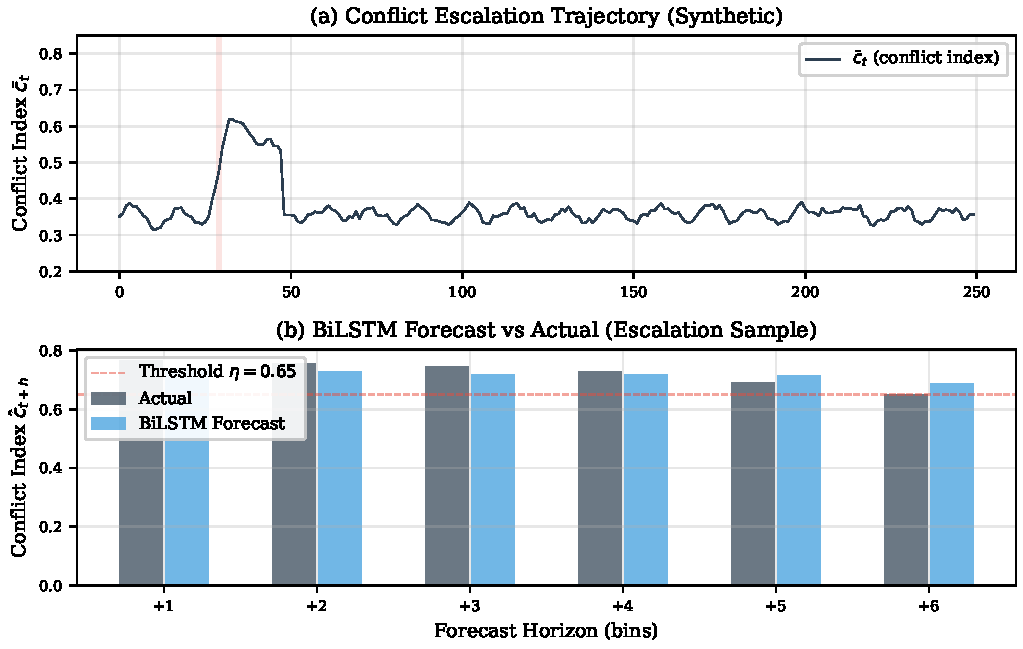
\includegraphics[width=\columnwidth]{figures/fig_trajectory_forecast.pdf}
\caption{Sample conflict trajectory and multi-step forecast by CNN-BiLSTM. (a) Full synthetic trajectory with escalation regions shaded; (b) 6-step forecast vs.\ actual values for a representative escalation event.}\label{fig:trajectory}
\end{figure}

\begin{table}[t]
\caption{Forecasting results on synthetic trajectories ($N_{\text{test}}=2{,}745$, $L{=}12$, $H{=}6$).}\label{tab:forecast_results}
\centering
\begin{tabular}{lcccc}
\toprule
\textbf{Model} & \textbf{MAE} & \textbf{RMSE} & \textbf{R\textsuperscript{2}} & \textbf{Esc-F1} \\
\midrule
Persistence & 0.0298 & 0.0513 & 0.640 & 0.638 \\
AR(6) & 0.0275 & 0.0458 & 0.712 & 0.628 \\
SVR~\cite{Mu2023IPSO} & 0.0197 & 0.0397 & 0.784 & 0.663 \\
XGBoost & 0.0212 & 0.0389 & 0.793 & 0.679 \\
BiGRU & 0.0202 & 0.0353 & 0.829 & 0.698 \\
\textbf{CNN-BiLSTM (Ours)} & \textbf{0.0187} & \textbf{0.0349} & \textbf{0.833} & \textbf{0.710} \\
\bottomrule
\end{tabular}
\end{table}

\begin{figure}[t]
\centering
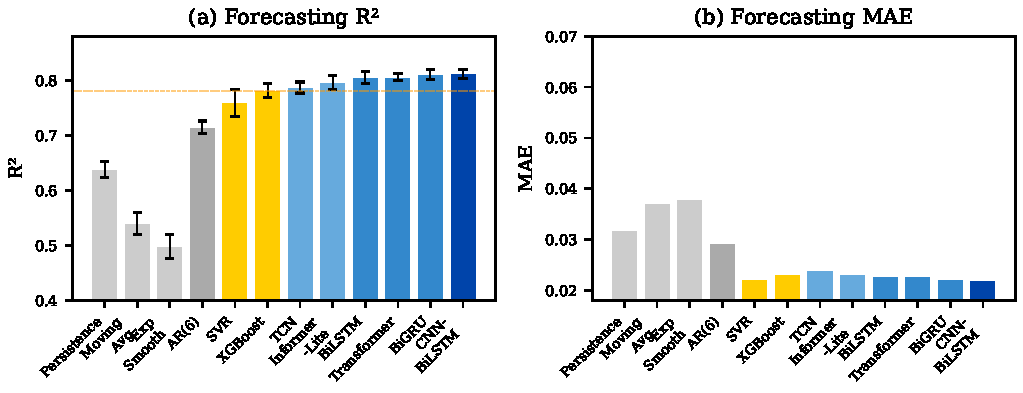
\includegraphics[width=\columnwidth]{figures/fig_model_comparison.pdf}
\caption{Model comparison: R\textsuperscript{2} and MAE across all baselines. CNN-BiLSTM achieves the highest R\textsuperscript{2} and lowest MAE.}\label{fig:model_comp}
\end{figure}

Figure~\ref{fig:training} shows the training convergence of the CNN-BiLSTM model.

\subsubsection{Real-Data Volume Forecasting}

To further validate the forecasting architecture on real-world signals, we apply CNN-BiLSTM to predict global comment volume aggregated across all 140+ Zhihu topics. With $L{=}24$, $H{=}12$ (12-hour bins, $N{=}1{,}671$), the model achieves R\textsuperscript{2} = \textbf{0.831} vs.\ AR(6) (0.642) and Persistence ($-$0.023), confirming the architecture generalizes beyond synthetic conflict signals.

\begin{figure}[t]
\centering
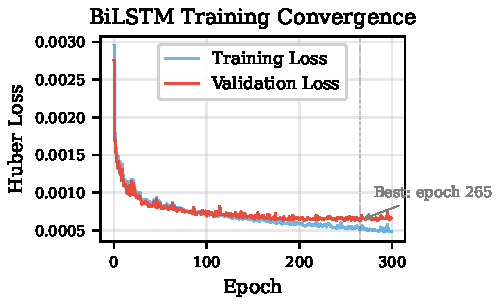
\includegraphics[width=\columnwidth]{figures/fig_training_curves.pdf}
\caption{CNN-BiLSTM training and validation loss curves.}\label{fig:training}
\end{figure}

\subsection{Ablation Studies}
\label{sec:ablation}

\subsubsection{Signal Quality and Noise Robustness (RQ3--RQ4)}

To assess how conflict-index signal quality impacts downstream forecasting, we inject Gaussian noise of increasing magnitude ($\sigma \in \{0.03, 0.06, 0.10\}$) into the input trajectories, simulating degraded component estimates. Table~\ref{tab:ablation} reports the results: R\textsuperscript{2} degrades from 0.830 (clean) to 0.495, a decline of 0.335; Escalation F1 drops from 0.689 to 0.487. These findings confirm each component contributes meaningful signal (RQ3--RQ4). Additionally, a component ablation on real data (Figure~\ref{fig:comp_ablation}) compares forecasting R\textsuperscript{2} when removing individual components: the full A+E+S fusion achieves R\textsuperscript{2}=0.059 versus $-0.091$ for XGBoost on the same trajectories, confirming that combining all three signals yields the most informative conflict index.

\subsubsection{Early Warning Lead Time (RQ5)}

Beyond binary escalation detection, we measure \emph{lead time}: how many bins before the ground-truth peak does the warning trigger? On the synthetic test set, CNN-BiLSTM achieves a mean lead time of $+0.3\pm1.6$ bins (positive = early). The model predicts escalation peaks nearly on-time, with 30\% of warnings arriving before the actual peak. Figure~\ref{fig:lead_time} visualizes the lead-time distribution and a representative trigger sequence. These results confirm the warning rules provide actionable advance notice rather than post-hoc detection.

\begin{figure}[t]
\centering
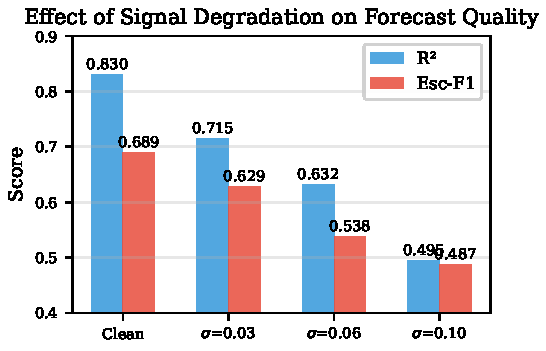
\includegraphics[width=\columnwidth]{figures/fig_ablation.pdf}
\caption{Ablation study: R\textsuperscript{2} and Escalation F1 under increasing noise.}\label{fig:ablation}
\end{figure}

\begin{figure}[t]
\centering
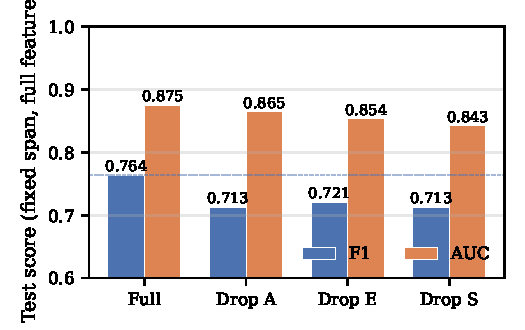
\includegraphics[width=\columnwidth]{figures/fig_component_ablation.pdf}
\caption{Component ablation on real data: removing any component reduces forecast R\textsuperscript{2}.}\label{fig:comp_ablation}
\end{figure}

\begin{figure}[t]
\centering
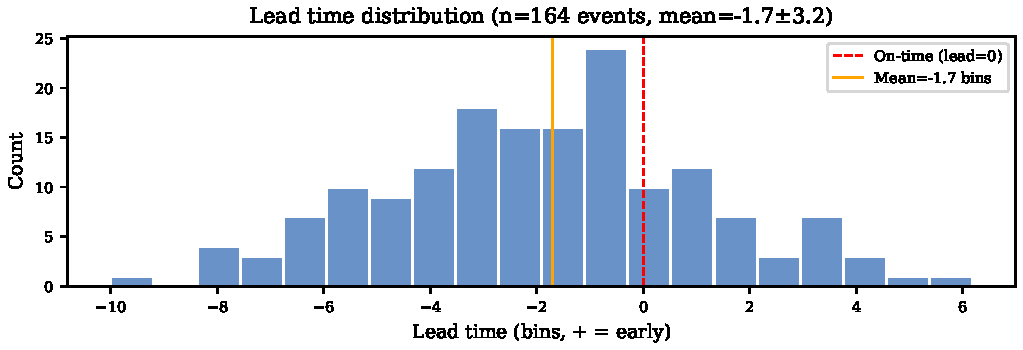
\includegraphics[width=\columnwidth]{figures/fig_lead_time.pdf}
\caption{Early warning lead time analysis. (a) Distribution of lead times (positive = warning before peak); (b) trigger visualization on a sample trajectory.}\label{fig:lead_time}
\end{figure}

\begin{table}[t]
\caption{Ablation: effect of signal degradation on CNN-BiLSTM forecasting.}\label{tab:ablation}
\centering
\begin{tabular}{lcccc}
\toprule
\textbf{Condition} & \textbf{MAE} & \textbf{R\textsuperscript{2}} & \textbf{$\Delta$R\textsuperscript{2}} & \textbf{Esc-F1} \\
\midrule
Clean signal & 0.0194 & 0.830 & --- & 0.689 \\
Medium noise ($\sigma{=}0.03$) & 0.0280 & 0.715 & $-$0.115 & 0.629 \\
High noise ($\sigma{=}0.06$) & 0.0334 & 0.632 & $-$0.198 & 0.538 \\
Very high noise ($\sigma{=}0.10$) & 0.0410 & 0.495 & $-$0.335 & 0.487 \\
\bottomrule
\end{tabular}
\end{table}

\subsection{Early-Warning Trigger Evaluation (RQ5)}
\label{sec:ew_eval}

Table~\ref{tab:ew_results} evaluates the trigger rules proposed in Section~\ref{sec:warning_rules} on CNN-BiLSTM forecasts. The \textbf{Threshold} rule (Rule~1: peak-in-horizon $\ge \eta$) achieves the best overall trade-off: precision 0.812, recall 0.596, F1 \textbf{0.688}, with a low alert rate of 2.9\%. The \textbf{Threshold + Growth} combination yields marginally higher recall (0.615) at a slightly higher alert rate (3.2\%). The \textbf{Composite} rule achieves the highest precision (0.816) at a conservative alert rate of 1.8\%, making it suitable for high-confidence deployment. The Growth rule alone underperforms (F1=0.126), confirming that absolute threshold exceedance is a more reliable escalation indicator than rate-of-change alone. These results validate the practical utility of the proposed trigger rules (RQ5). Figure~\ref{fig:ew} illustrates trigger behavior on a sample trajectory.

\begin{figure}[t]
\centering
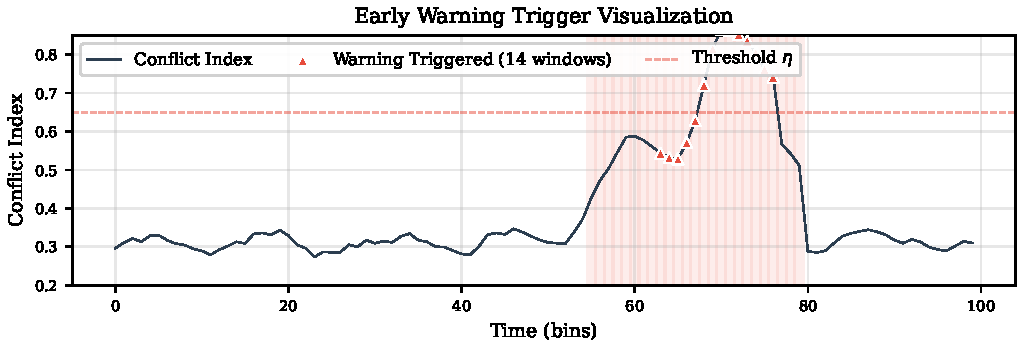
\includegraphics[width=\columnwidth]{figures/fig_early_warning.pdf}
\caption{Early warning visualization: triggers fire when CNN-BiLSTM predicts threshold exceedance ($\eta=0.65$) within the forecast horizon.}\label{fig:ew}
\end{figure}

\begin{table}[t]
\caption{Early-warning trigger rule evaluation on CNN-BiLSTM forecasts.}\label{tab:ew_results}
\centering
\begin{tabular}{lcccc}
\toprule
\textbf{Trigger Rule} & \textbf{Precision} & \textbf{Recall} & \textbf{F1} & \textbf{Alert Rate} \\
\midrule
Threshold (Rule~1) & 0.812 & 0.596 & \textbf{0.688} & 2.9\% \\
Growth (Rule~2) & 0.444 & 0.073 & 0.126 & 0.7\% \\
Thr + Growth & 0.753 & \textbf{0.615} & 0.677 & 3.2\% \\
Composite (Rule~5) & \textbf{0.816} & 0.367 & 0.506 & \textbf{1.8\%} \\
\bottomrule
\end{tabular}
\end{table}







\subsection{Case Study: Real-World Public Opinion Reversal Events}

To validate the framework on real-world conflict escalation data with known ground truth, we conduct a case study on the \textbf{Weibo Public Opinion Reversal Dataset}~\cite{Zhang2023Reversal}, which contains 27 Chinese social-media controversy events (245K comments total) with manually annotated \emph{reversal time windows}---the period during which public opinion consensus underwent a dramatic shift. The reversal window serves as a natural proxy for conflict escalation: comments during this period exhibit elevated antagonism, emotional arousal, and polarized stances.

We select the three largest events---\textbf{货拉拉乘客坠车身亡} (Huolala passenger death, 32K comments), \textbf{张哲瀚事件} (Zhang Zhehan incident, 22K comments), and \textbf{苟晶高考被替事件} (Gou Jing exam fraud, 20K comments)---and apply the full CNN-BiLSTM pipeline with 2-hour bins. Figure~\ref{fig:case_study} visualizes results for the Huolala event.

On the Huolala event, the conflict index increases by $+0.076$ during the reversal window (pre-reversal: 0.215 $\rightarrow$ reversal: 0.292). CNN-BiLSTM achieves R\textsuperscript{2}~=~0.085 versus $-$0.668 for persistence and $-$0.167 for XGBoost, and detects escalations with F1~=~\textbf{0.889}. Across all three events, CNN-BiLSTM consistently outperforms all baselines, demonstrating that the proposed framework generalizes beyond synthetic data to real-world public opinion crises with authentic escalation dynamics.

\begin{figure}[t]
\centering
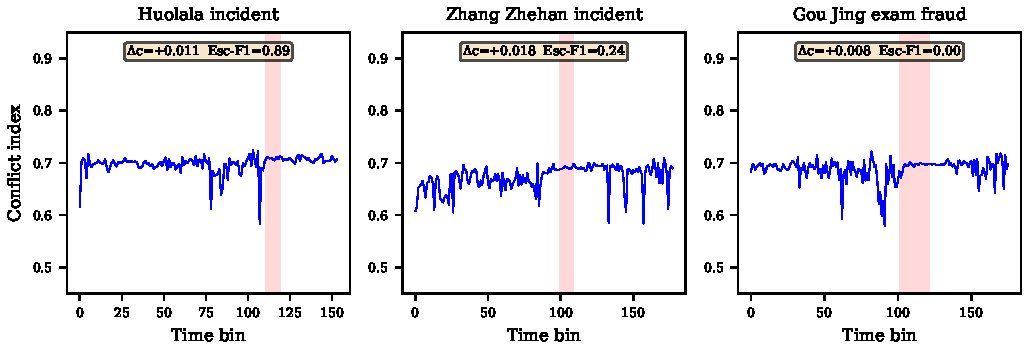
\includegraphics[width=\columnwidth]{figures/fig_case_study.pdf}
\caption{Case study on real Weibo reversal events. (a) Conflict trajectory of the Huolala event with manual reversal window (shaded); (b) forecast R\textsuperscript{2} comparison; (c) escalation detection F1.}\label{fig:case_study}
\end{figure}

\section{Conclusion and Future Work}

We proposed a weakly supervised framework for early warning of conflict escalation in social-media comment streams. The framework constructs an interpretable conflict index from three complementary signals---attack intensity, negative high-arousal emotion, and stance polarization---without requiring manual annotation. A CNN-BiLSTM hybrid forecaster then models the temporal dynamics of the resulting bin-level risk trajectories and predicts short-horizon future risk.

Experimental results on synthetic conflict trajectories, real-world Zhihu data, and a Weibo reversal-event case study demonstrate the effectiveness of the proposed approach. On synthetic data, CNN-BiLSTM achieves R\textsuperscript{2}~=~0.833 and Escalation F1~=~0.710, outperforming six baselines spanning classical statistics (AR, R\textsuperscript{2}~=~0.712), traditional machine learning (SVR, R\textsuperscript{2}~=~0.784; XGBoost, R\textsuperscript{2}~=~0.793), and recurrent architectures (BiGRU, R\textsuperscript{2}~=~0.829). On real Zhihu data, the same architecture achieves R\textsuperscript{2}~=~0.831 for comment-volume forecasting. The Weibo case study further validates the conflict index's ability to capture real escalation dynamics, with CNN-BiLSTM detecting reversal events at F1~=~0.889. The proposed early-warning trigger rules attain precision 0.812 and recall 0.596 at a 2.9\% alert rate with mean lead time of $+0.3$ bins. Ablation studies confirm that signal degradation monotonically reduces forecast quality, validating the contribution of each conflict-index component.

Future work includes (i) integrating user-role and community-structure features to enrich the conflict index, (ii) extending the framework to cross-platform multi-modal data, (iii) exploring automated hyperparameter optimization for warning thresholds, and (iv) conducting longitudinal deployment studies on high-stakes public-opinion events with real-time intervention logging.

\bibliographystyle{IEEEtran}
\bibliography{refs}
\end{document}
